%----------------------------------------------------------------------------------------
%	GOALS
%----------------------------------------------------------------------------------------

\section{Konzeption des Prototyps}

%------------------------------------------------

\subsection{Datenmodellierung}
\label{sec:datastructures}

Die zentrale Datenstruktur der Applikation ist die Beschreibung der API selbst, welche als Grundlage für alle Operationen verwendet wird. Da sich der Prototyp beim Eingabeformat auf das OpenAPI Spezifikationsformat beschränkt, wurde zunächst ein OpenAPI Metamodell erstellt, welches in Abbildung \ref{fig:openapi} dargestellt ist. Dieses Modell wird von der Applikation als Basis-Datenstruktur verwendet. Zur Unterstützung mehrerer Eingabeformate müssten in einer späteren Iteration auch andere Spezifikationsformate untersucht werden, um Gemeinsamkeiten abzuleiten und ein Datenmodell zu erstellen, in das alle Formate überführt werden können. \\

\begin{figure}
  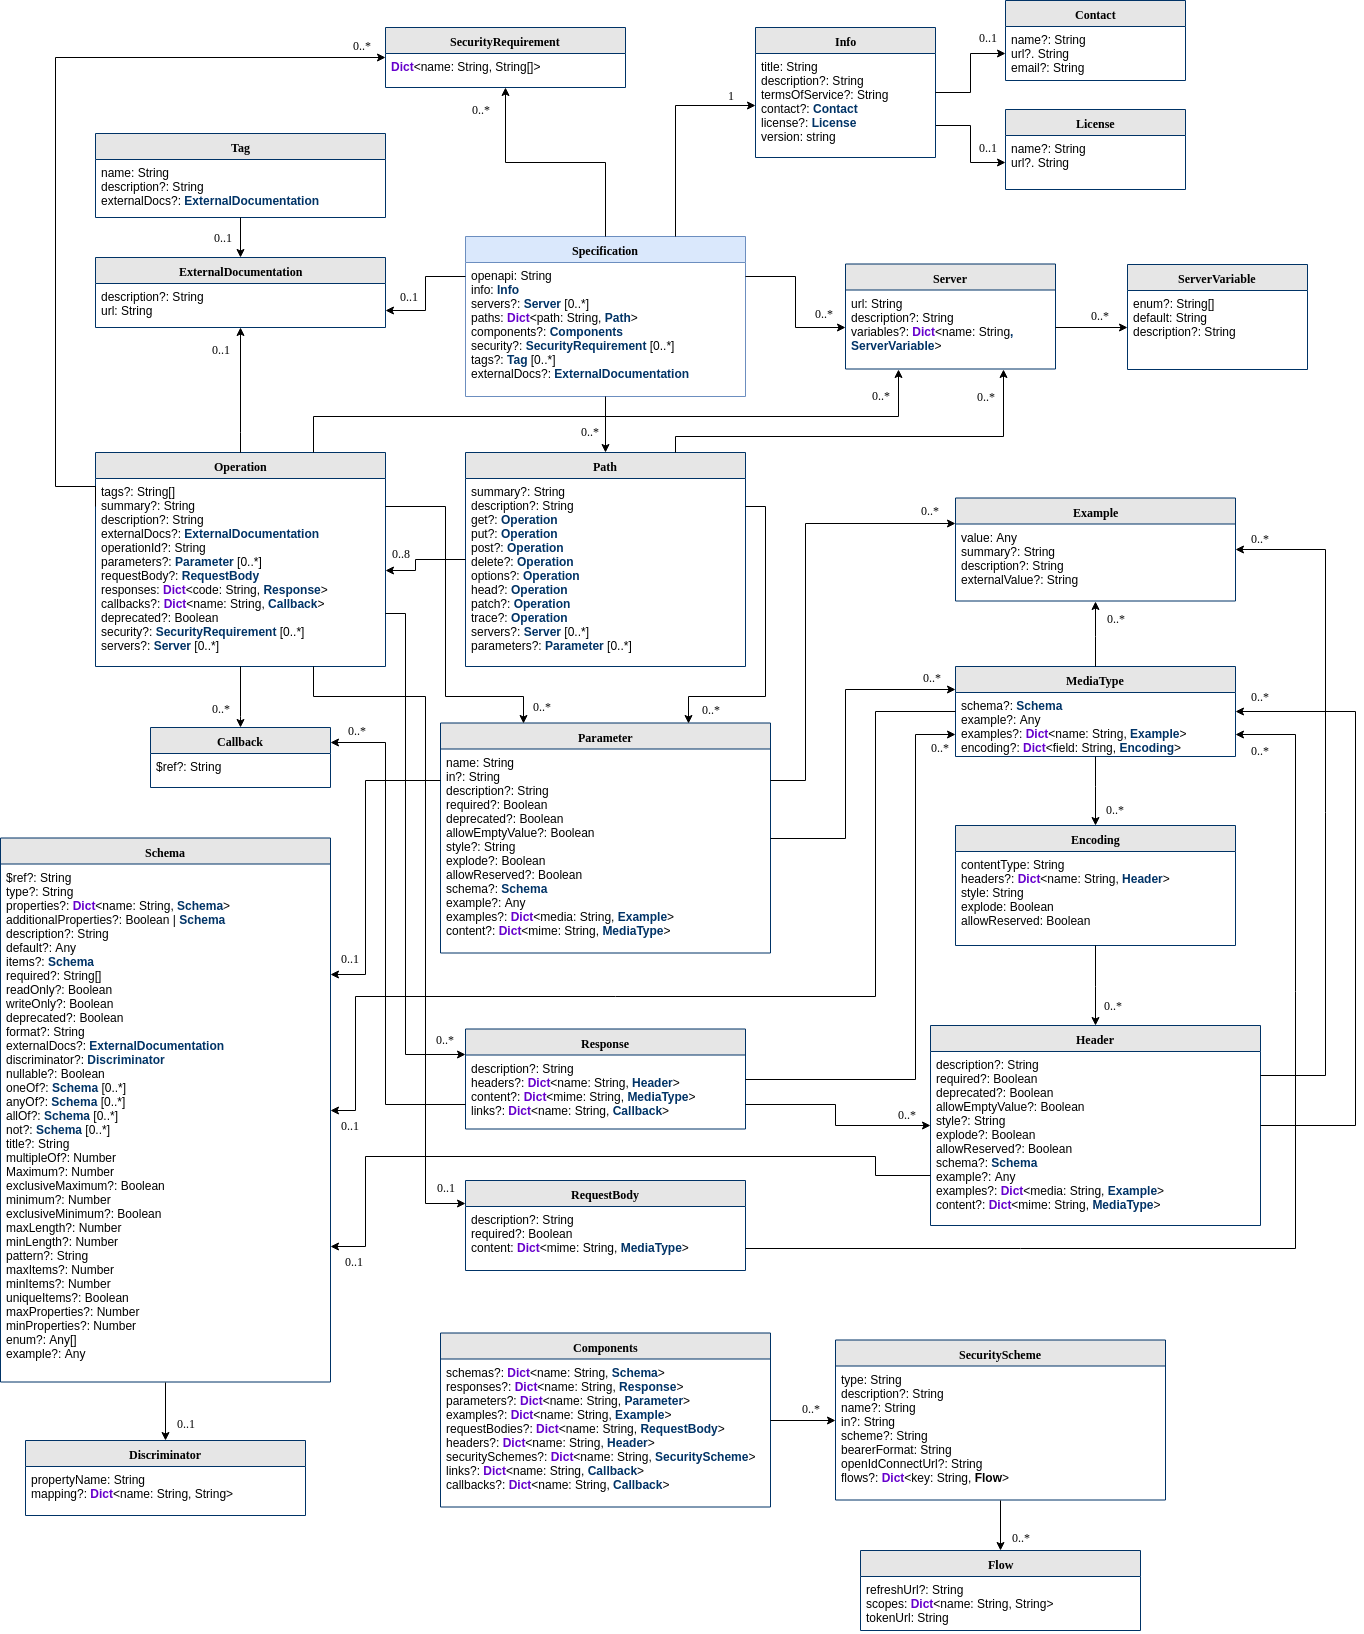
\includegraphics[width=\textwidth,height=\textheight,keepaspectratio]{../images/open-api.png}
  \caption{OpenAPI Metamodell}
  \label{fig:openapi}
\end{figure}

Es wurden ebenfalls zwei weitere Datenmodelle erstellt, die für die im Prototyp festgelegten Ziele benötigt werden. Zunächst wurde ein Modell der JSON-Schema Spezifikation erstellt, welche sich nur in wenigen Divergenzen von der OpenAPI Schema Definition unterscheidet:

\begin{enumerate}
	\item Einige im OpenAPI Schema vorhandene Attribute wie \lstinline|nullable| oder \lstinline|deprecated| werden nicht unterstützt.
	\item Die \lstinline|type| Angabe kann sowohl ein String wie auch ein Array von Strings sein.
	\item in \lstinline|$schema| wird zusätzlich ein Link zur verwendeten JSON-Schema Version angegeben. 
\end{enumerate}

Diese Unterschiede müssen bei einer Umwandlung rekursiv aufgelöst werden, da ein Schema weitere verschaltete Schema-Defitionen enthalten kann. Das Modell einer JSON-Schema Definition ist in Abbildung \ref{fig:jsonschema} dargestellt. \\

\begin{figure}
\centering
  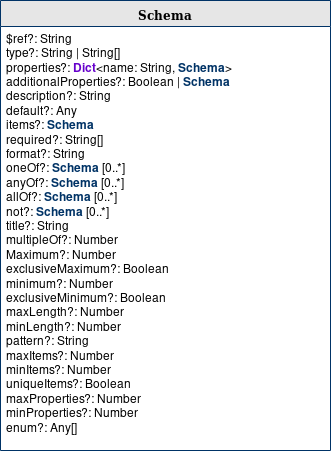
\includegraphics[width=0.5\textwidth]{../images/json-schema.png}
  \caption{JSON-Schema Metamodell}
  \label{fig:jsonschema}
\end{figure}

Das Testsuite-Metamodell (Abbildung \ref{fig:testsuite}) stellt den Aufbau einer Testsuite dar, welche aus mehreren  Testcases besteht. In jedem Testcase wird eine Anfrage mit entsprechenden Parametern ausgeführt, sowie eine Reihe von Assertions:

\begin{enumerate}
	\item \lstinline|ValidStatusCodeAssertion| prüft, ob der HTTP-Statuscode der erhaltenen Antwort valide ist. Bei nominalen Testcases wird ein erfolgreicher Statuscode (2xx) erwartet, bei fehlerhaften Testcases ein Client-Fehler (4xx).
	\item \lstinline|HeaderExistsAssertion| prüft, ob alle in der Spezifikation definierten HTTP-Header vorhanden sind.
	\item \lstinline|ValidHeaderAssertion| prüft, ob alle HTTP-Header valide Werte haben.
	\item \lstinline|SchemaComplianceAssertion| validiert die vom Server erhaltene Antwort mit dem passenden JSON-Schema.
\end{enumerate}

Ein Testcase führt ebenfalls mehrere Hooks aus, die von dem Entwickler angepasst werden können. Dadurch kann zum Beispiel Authentifizierung ermöglicht werden.

\begin{figure}
\centering
  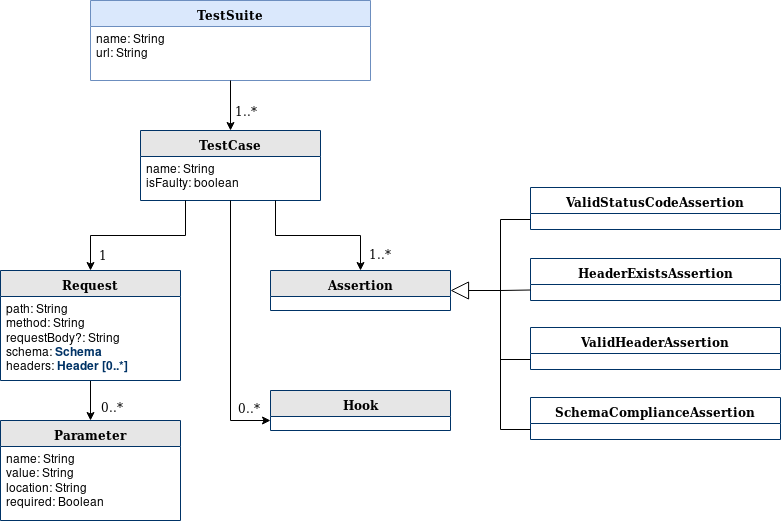
\includegraphics[width=\textwidth]{../images/testsuite.png}
  \caption{Testsuite Metamodell}
  \label{fig:testsuite}
\end{figure}


%------------------------------------------------

\subsection{Architektur}

Unter Berücksichtigung der beiden Ziele \textbf{Modularität} und \textbf{einfache Einbindung in Projekte} wird für die Umsetzung eine Javascript CLI-Applikation entwickelt. In den meisten Projekten sind bereits Javascript-Abhängigkeiten installiert, sodass sich das Tool leicht einbinden lässt. Durch NPM und die Aufteilung der Applikation in einzelne Pakete mit dynamischen Imports lässt sich ebenfalls die Modularität erreichen.\\

Die CLI-Applikation besteht aus einer Menge an Befehlen, welche alle den gleichen Aufbau haben, schematisch dargestellt in Abbildung \ref{fig:architecture}. Jeder Befehl besteht aus einem \emph{Parser}, der die API Spezifikation einliest, einem oder mehreren \emph{Decorators}, welche die geparste Spezifikation mit befehlspezifischer Logik und Informationen anreichern, sowie einer oder mehreren \emph{Factories}, die einen Output generieren. \\

\begin{figure}[H]
\centering
  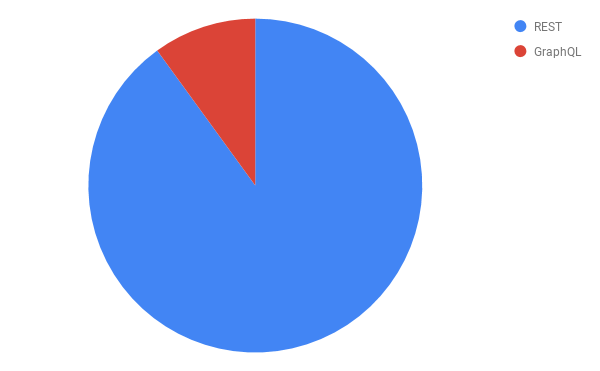
\includegraphics[width=\textwidth]{../images/architecture.png}
  \caption{Architektur}
  \label{fig:architecture}
\end{figure}

Diese Komponenten sind beliebig austauschbar und konfigurierbar. Dadurch wird ermöglicht, dass bei Änderungen am Input- oder Output-Format die restliche Logik nicht verändert werden muss. So können z.B. mithilfe von 2 Factories Tests für zwei unterschiedliche Sprachen oder Frameworks generiert werden, ohne dass etwas an dem Parsing oder Anreichern der Daten (im Falle der Tests z.B. das Ableiten von Parameter-Werten) verändert werden muss. Durch dynamische Imports mithilfe eines \emph{Resolvers} werden die einzelnen Pakete zur Laufzeit eingebunden. Somit können Entwickler auch eigene Pakete erstellen, die dann von der Applikation verwendet werden können. Da Javascript keine Interfaces unterstützt, wird stattdessen Typescript für die Implementierung verwendet. Damit kann sichergestellt werden, dass Entwickler auf fest definierte Interfaces und Typdefinitionen zurückgreifen können, an die sich ihre Pakete halten müssen. 


%------------------------------------------------

\subsection{Vorgehensmodell}
In folgendem Abschnitt wird kurz auf die Vorgehensweise der zwei Befehle \lstinline|make:schemas| und \lstinline|make:tests| eingegangen, welche im Prototyp der Applikation umgesetzt werden sollen. 

\subsubsection{Generierung von JSON Schemas}
Zur Generierung der JSON Schemas werden ein \emph{Decorator} und eine \emph{Factory} implementiert:

\begin{itemize}
	\item \textbf{Decorator}: der Decorator iteriert über alle Endpunkte und darin definierte Request- und Response-Bodies, und wandelt, falls vorhanden, die jeweiligen Open-API Schema Definitionen in valide JSON Schemas um. Dafür werden die bereits in Abschnitt \ref{sec:datastructures}[3.1] beschriebenen Unterschiede berücksichtigt. Anschließend werden die erstellten JSON Schemas der API Spezifikation hinzugefügt.
	\item \textbf{Factory}: die Factory schreibt die generierten JSON Schemas in \lstinline|json|-Dateien in den konfigurierten Output-Ordner, und verwendet dabei einfach verständliche Dateinamen. So wird das JSON Schema der Anfrage eines HTTP \lstinline|PATCH| Aufrufs auf die Ressource \lstinline|/books| z.B. in \lstinline|requests/books-update.json| gespeichert.
\end{itemize}

\subsubsection{Generierung von Testcases}
Zur Generierung von Testcases werden ebenfalls ein neuer \emph{Decorator} und eine \emph{Factory} implementiert. Der Befehl benutzt außerdem den bereits für JSON Schemas definierten \emph{Decorator}, da in den Tests die Antworten vom Server mithilfe von JSON Schemas validiert werden.

\begin{itemize}
	\item \textbf{Decorator}: der Decorator der Decorator iteriert über alle Endpunkte und erstellt das in Abbildung \ref{fig:testsuite} definierte Testsuite Modell. Für jede Anfrage werden mithilfe von verschiedenen Heuristiken Parameterwerte abgeleitet, die in den Testanfragen benutzt werden können. Die hierfür verwendeten Heuristiken basieren auf den bereits in \textcite{ed2018automatic} definierten Heuristiken, wurden jedoch für eine erhöhte Genauigkeit noch angepasst bzw. erweitert und an die aktuelle Syntax der OpenAPI v3.0.2. Spezifikation angepasst: 
	\begin{enumerate}
		\item Der Wert eines Parameters \lstinline|p| kann abgeleitet werden aus: Beispielwerten (\lstinline|p.example|, \lstinline|p.examples|, \lstinline|p.schema.example|, \lstinline|p.content.example|, \lstinline|p.content.examples| oder \lstinline|p.content.schema.example|), Standardwerten (\lstinline|p.schema.default|, \lstinline|p.schema.items.default| wenn \lstinline|p| vom Typ \lstinline|array| ist, \lstinline|p.content.schema.default| oder \lstinline|p.content.schema.items.default|) oder Enums (\lstinline|p.schema.enum|,  \lstinline|p.items.enum| wenn \lstinline|p| vom Typ \lstinline|array| ist, \lstinline|p.content.schema.enum| oder \lstinline|p.content.schema.items.enum|).
		\item Der Wert eines Parameters kann abgeleitet werden, wenn eine Anfrage mit einem automatisch generierten Wert (bspw. ein String wenn der Parameter vom Typ \lstinline|string| ist) erfolgreich ist.
		\item Der Wert eines Parameters kann abgeleitet werden, wenn für die selbe Ressource in einer der vorhanden Operationen ein Attribut gleichen Namens im Schema der Antwort definiert ist.
	\end{enumerate}
	Für fehlerhafte Testcases müssen fehlerhafte Parameter bzw. Attribut-Werte abgeleitet werden, was mithilfe verschiedener Regeln basierend auf dem Typ und den im Schema definierten Einschränkungen möglich ist, aufgelistet in den Tabellen \ref{tab:types} und \ref{tab:constraints}. 
	\item \textbf{Factory}: die Factory generiert die einzelnen Testcases in einer bestimmten Zielsprache. Dafür werden die in den Decorators angelegten Parameterwerte und JSON Schemas verwendet. Für jede API Operation wird, wenn für alle erfoderlichen Parameter (\lstinline|p.required = true|) Werte abgeleitet werden konnten,  für jede mögliche Parameterkombination ein separates Testcase erstellt, in dem eine Anfrage an den Server mit den abgeleiteten Parameterwerten geschickt wird. Anschließend wird geprüft, dass die Antwort einen validen Statuscode hat (2xx bei nominalen Testcases bzw. 4xx bei fehlerhaften Testcases), und mit den generierten JSON Schemas validiert werden kann. Über \emph{Hooks}, die bei jedem Testcase vor und nach dem Ausführen der Anfrage aufgerufen werden, kann der Entwickler Anpassungen vornehmen. So kann z.B. Authentifizierung ermöglicht werden. 
\end{itemize}

\begin{table}[]
\centering
\caption{Datentypen}
\label{tab:types}
\begin{tabular}{|l|l|}
\hline
\textbf{Typ}                                                      & \textbf{Regel}                                           \\ \hline
\lstinline|object|                                                   & Ein Objekt, welches das Schema verletzt         \\ \hline
\begin{tabular}[c]{@{}l@{}}\lstinline|integer|\\ \lstinline|number|\end{tabular} & Zufälliger String der keine Zahlen enthält      \\ \hline
\lstinline|boolean|                                                  & Zufälliger String der nicht \lstinline|true|  oder \lstinline|false|  ist \\ \hline
\end{tabular}
\end{table}

\begin{table}[!t]
\centering
\caption{Einschränkungen}
\label{tab:constraints}
\begin{tabular}{|l|l|}
\hline
\textbf{Einschränkung} & \textbf{Regel}                                             \\ \hline
\lstinline|enum|                                                                                                                               & String oder Zahl, die nicht im Enum enthalten ist \\ \hline
\lstinline|maximum / exclusiveMaximum                                                                                                        | & Integer, der größer als das Maximum ist           \\ \hline
\lstinline|minimum / eclusiveMinimum                                                                                                         |                                                                                                                               & Integer, der kleiner als das Minimum ist          \\ \hline
\lstinline|minLength|                                                                                                                                                                                                                                                        & String, der kürzer als \lstinline|minLength|                                                                                                                                                                                                                                                         ist              \\ \hline
\lstinline|maxLength|                                                                                                                                                                                                                                                        & String, der länger als \lstinline|maxLength|                                                                                                                                                                                                                                                        ist              \\ \hline
\lstinline|maxItems|                                                                                                                                                                                                                                                         & Array mit mehr Items als \lstinline|maxItems|                                                                                                                                                                                                                                                                        \\ \hline
\lstinline|minItems|                                                                                                                                                                                                                                                         & Array mit weniger Items als \lstinline|minItems|                                                                                                                                                                                                                                                                      \\ \hline
\begin{tabular}[c]{@{}l@{}}\lstinline|format:date-time|                                                                                                                                                                                                                                                        \\ \lstinline|format:email|                                                                                                                                                                                                                                                                     \\ \lstinline|format:hostname|                                                                                                                                                                                                                                                                     \\ \lstinline|format:ipv4|                                                                                                                                                                                                                                                                     \\ \lstinline|format:ipv6|                                                                                                                                                                                                                                                                     \\ \lstinline|format:uri|                                                                                                                                                                                                                                                                     \end{tabular} & Zufälliger String aus \lstinline|[A-Za-z]|                                                                                                                                                                                                                                                                                    \\ \hline
\end{tabular}
\end{table}